\documentclass[../main.tex]{subfiles}
% !TEX root= ../main.tex

\begin{document}

\subsection{The MESI protocol}

\begin{center}
	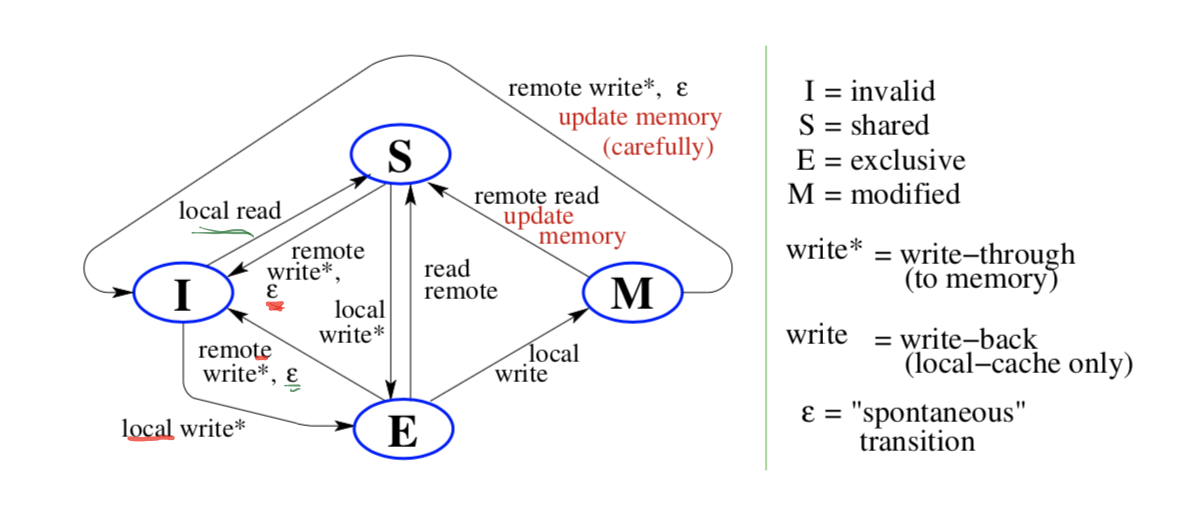
\includegraphics[scale=0.65]{mesi.png}
\end{center}

\begin{itemize}
	\item \textbf{Write-back:} writes only update the cache, main memory updated when the cache block is evicted.
	\item \textbf{Write-through:} writes update cache and main-memory.
\end{itemize}

\begin{itemize}
	\item Caches can \textbf{shared read-only} copies of a cache block.
	\item When a processor writes a cache block, the \textbf{first write} goes to main memory
	      \begin{itemize}
		      \item The other caches are notified and invalidate their copies.
		      \item This ensures that writeable blocks are exclusive.
	      \end{itemize}
	\item MESI guarantees \textbf{sequential consistency}.
	      \begin{itemize}
		      \item All memory reads and writes from all processors can be arranged into a single, sub-sequential order.
	      \end{itemize}
	\item \textbf{Weak Consistency:} Reads can move ahead of writes to maximize program performance.
\end{itemize}

\subsubsection{Implementing MESI: Snooping}

\begin{itemize}
	\item Caches read and write main memory over a shared memory bus.
	\item Each cache has two copies of the tag: one for the CPU, the other for the bus.
	\item If the cache sees another CPU reading or writing block that is in this cache, it takes the action specified by the MESI protocol.
\end{itemize}

\subsubsection{Implementing MESI: Directories}

\begin{itemize}
	\item Main memory keeps a copy of the data and
	      \begin{itemize}
		      \item a bit-vector that record which processors have copies, and
		      \item a bit to indicate that one processor has a copy and it may be modified
	      \end{itemize}
	\item A processor accesses main memory as required by the MESI protocol.
	      \begin{itemize}
		      \item The memory unit sends messages to the other CPUs to direct them to take actions as needed by the protocol
		      \item The ordering of these messages ensures that memory stays consistent.
	      \end{itemize}
\end{itemize}

\subsubsection{Comparison}
\begin{itemize}
	\item Snooping is simple for machines with a small number of processors.
	\item Directory methods scale better to large numbers of processors.
\end{itemize}

\end{document}
